\section*{Anlage 4: Häufigkeiten der Verzierungselemente der Gefäßzonen bei Keramik der aufgenommen Stilgruppen}\label{sec:StilGrVerzMatrizen}
%\addcontentsline{toc}{chapter}{Verteilungs-Muster der Verzierungselemente}
\sectionmark{Anlage 4: Häufigkeiten der Verzierungselemente}

Die Aufnahme der Verzierungselemente (Tab.~\ref{tab:Verzierungselemente}) erfolgte differenziert nach der Position am Gefäß (Abb.~\ref{fig:Keramik_VerzZonen}; Kap.~\ref{sec:GefKeramik}). Auf Basis der so gewonnen Daten lassen sich für die keramischen Stilgruppen (siehe Kap.~\ref{sec:StilGr_nwCongo}) individuelle Häufigkeitstabellen erzeugen, die über die jeweiligen Verzierungspräferenzen Aufschluss geben. Im Folgenden finden sich diese umfassenden Tabellen: in den Zeilen die Gefäßposition und als Spalten die Verzierungselemente. Die Zellenwerte entsprechen gerundeten Prozentangaben, um die unterschiedliche Stichprobengröße auszugleichen.

\vspace{1em}\noindent Liste der Verzierungstechniken nach \textcite[44 Tab.~3; siehe Tab.~\ref{tab:Verzierungselemente}, Abb.~\ref{fig:Keramik_VerzSystematik}]{Wotzka.1995}:
$\;$ \\

\vspace{.5em}

\begin{center}
\noindent{\footnotesize
	\begin{sftabular}{@{}ll@{}}
		\toprule
		\textbf{Kürzel} & \textbf{Verzierung} \\
		\midrule
		01 & Ritzung \\
		02 & Riefung \\
		03 & Dellung/Fingereindruck \\
		04 & Eindruck/Stempel/Stich \\
		05 & Zahnstock- beziehungsweise Kammeindruck \\
		06 & Kerbschnitt \\
		07 & - \\
		08 & \textit{banfwa-nfwa} \\
		09 & Plastische Ornamente/Appliqué \\
		10 & - \\
		11 & Glättung (eingeglättete Verzierung) \\
		12 & Matten-/Korbgeflechtabdruck \\
		13 & Bohrung/Lochung/Ausgeschnittenes Ornament \\
		14 & Bemalung \\
		15 & Kammstrich \\
		16 & Textilabdruck \\
		17 & Handhaben \\
		18 & Netzabdruck \\
		19 & - \\
		20 & Sonstige \\
		21.1--4 & Vegetabilische \mbox{Roulette} \\
		21.5--13 & Schnitzroulette \\
		22.1--2 & Aufträge \& Aufrauung \\
		99 & Komplexe / kombinierte Techniken \\
		\bottomrule
	\end{sftabular}
}	
\end{center}

\begin{sidewaysfigure*}[p]

% Nummerierung dieser Sub-Anlagen anstatt Buchstaben!!! >> 4.1 -- 4.26
%\renewcommand{\thesubfigure}{\arabic{subfigure}}

\begin{subfigure}{\textwidth}
	\centering
	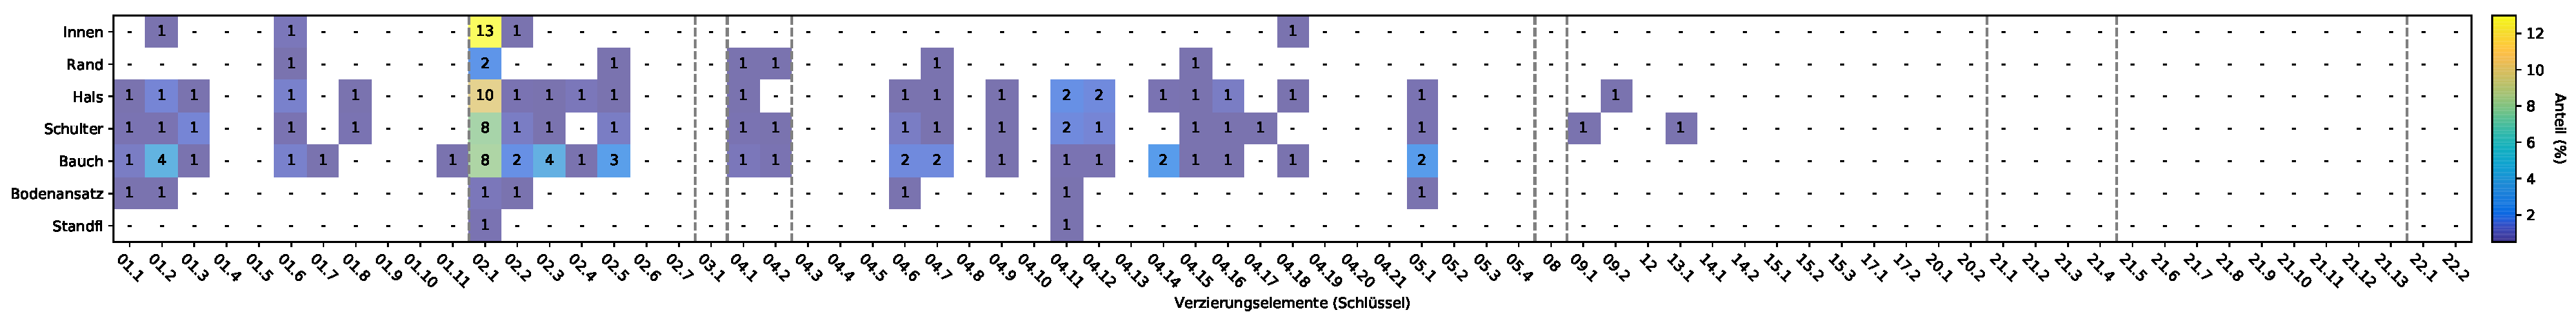
\includegraphics[width=\textwidth]{fig/BTM_Verzierungselmente.pdf}
	\caption*{\textbf{1}\hspace{1em}Batalimo-Maluba-Gruppe. \vspace{\baselineskip}}
	\label{fig:BatMLB_Verz}
\end{subfigure}

\begin{subfigure}{\textwidth}
	\centering
	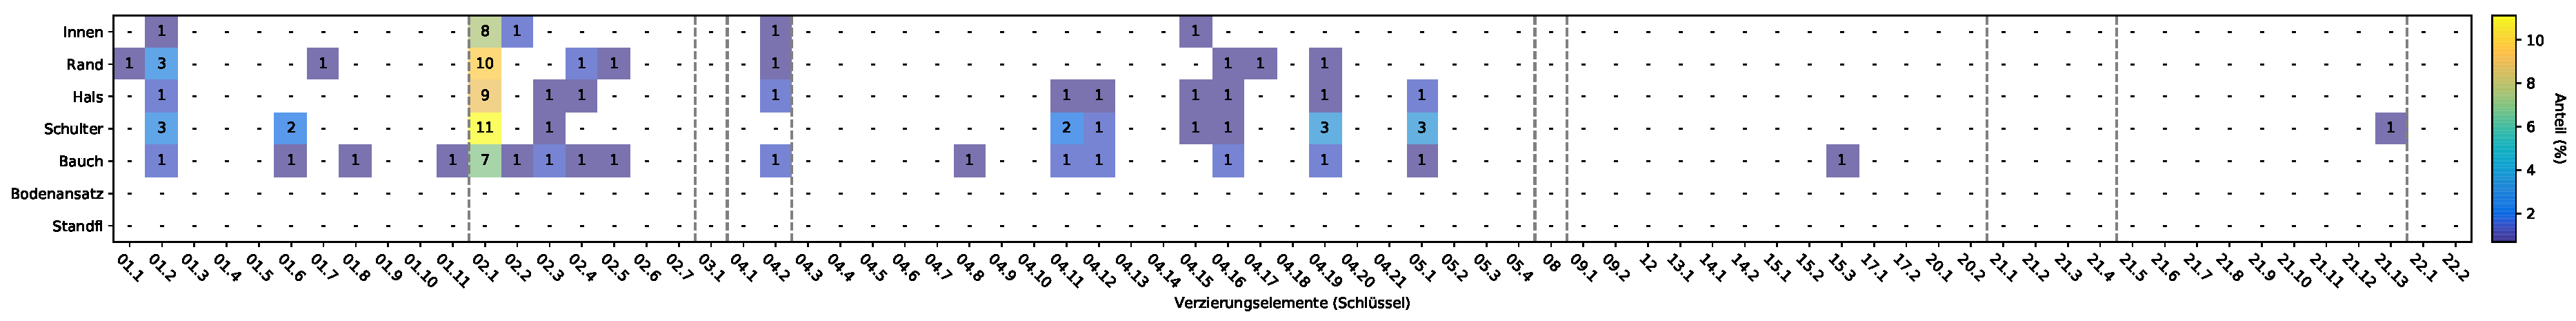
\includegraphics[width=\textwidth]{fig/NGB_Verzierungselmente.pdf}
	\caption*{\textbf{2}\hspace{1em}\mbox{Ngbanja}-Gruppe. \vspace{\baselineskip}}
	\label{fig:NGB_Verz}
\end{subfigure}

\begin{subfigure}{\textwidth}
	\centering
	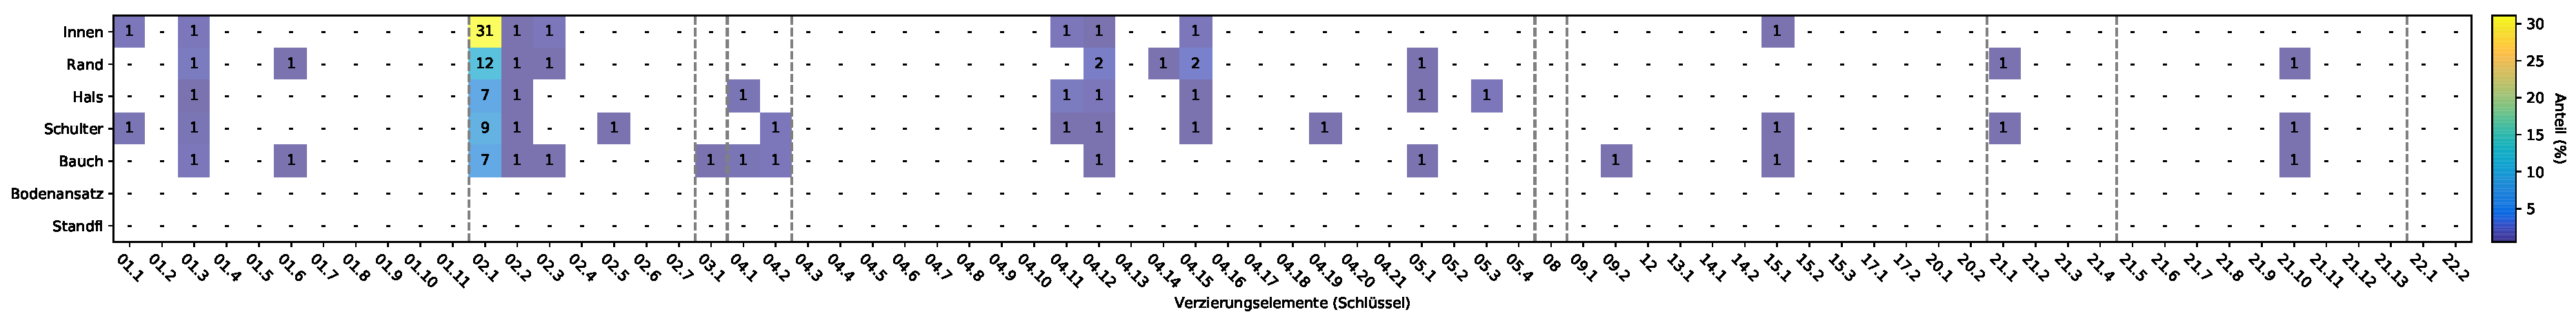
\includegraphics[width=\textwidth]{fig/DON_Verzierungselmente.pdf}
	\caption*{\textbf{3}\hspace{1em}Dongo-Gruppe. \vspace{\baselineskip}}
	\label{fig:DON_Verz}
\end{subfigure}
%\caption{Verzierungselemente: Häufigkeiten.}

\end{sidewaysfigure*}

\addtocounter{figure}{-1}
\begin{sidewaysfigure*}[p]

\begin{subfigure}{\textwidth}
	\setcounter{subfigure}{3}
	\centering
	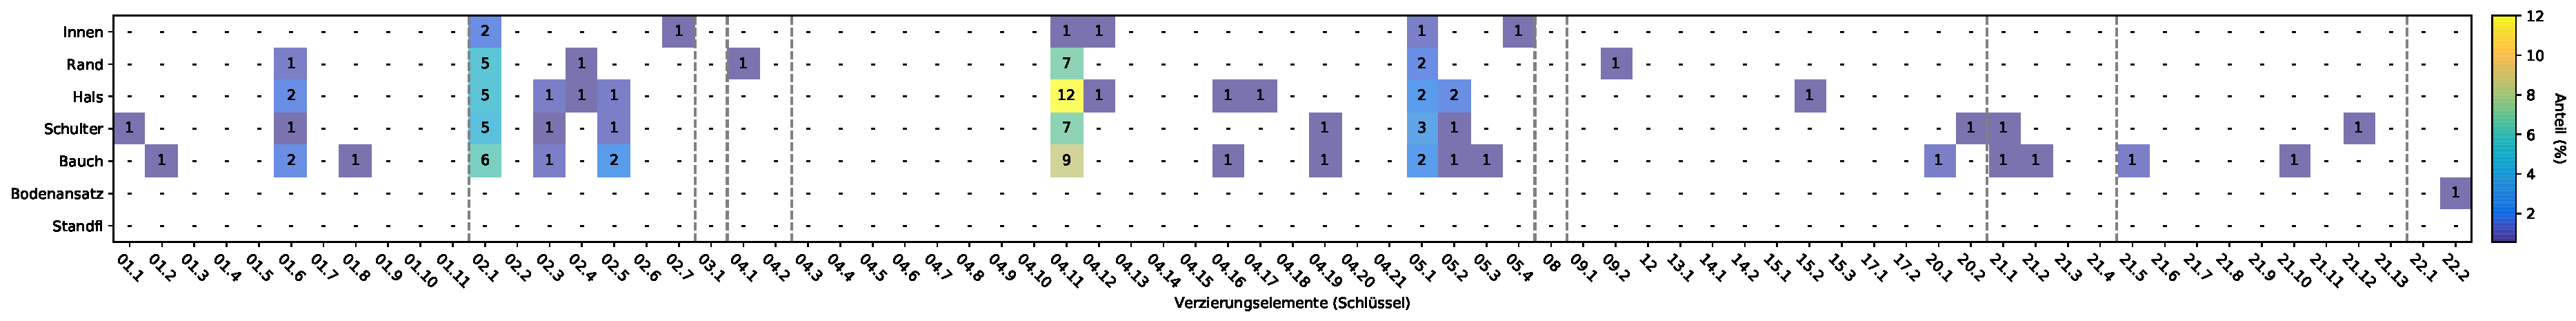
\includegraphics[width=\textwidth]{fig/MKL_Verzierungselmente.pdf}
	\caption*{\textbf{4}\hspace{1em}Mokelo-Gruppe. \vspace{\baselineskip}}
	\label{fig:MKL_Verz}
\end{subfigure}

\begin{subfigure}{\textwidth}
	\centering
	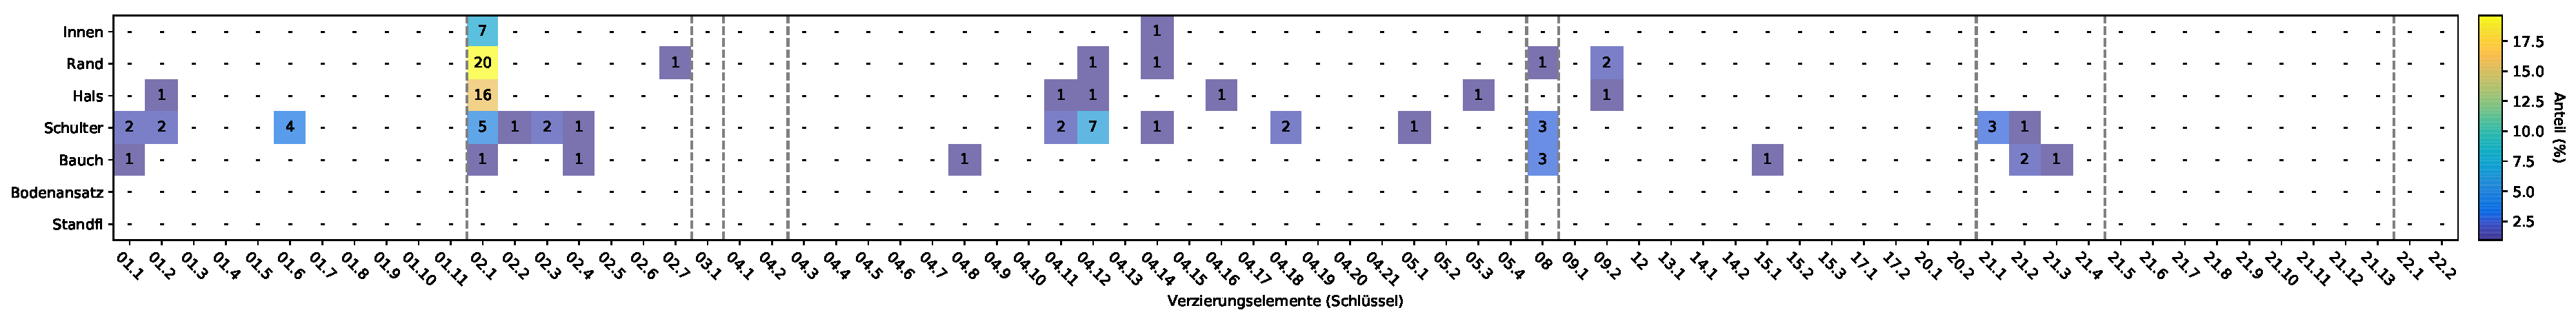
\includegraphics[width=\textwidth]{fig/BBL_Verzierungselmente.pdf}
	\caption*{\textbf{5}\hspace{1em}Bobulu-Gruppe. \vspace{\baselineskip}}
	\label{fig:BBL_Verz}
\end{subfigure}

\begin{subfigure}{\textwidth}
	\centering
	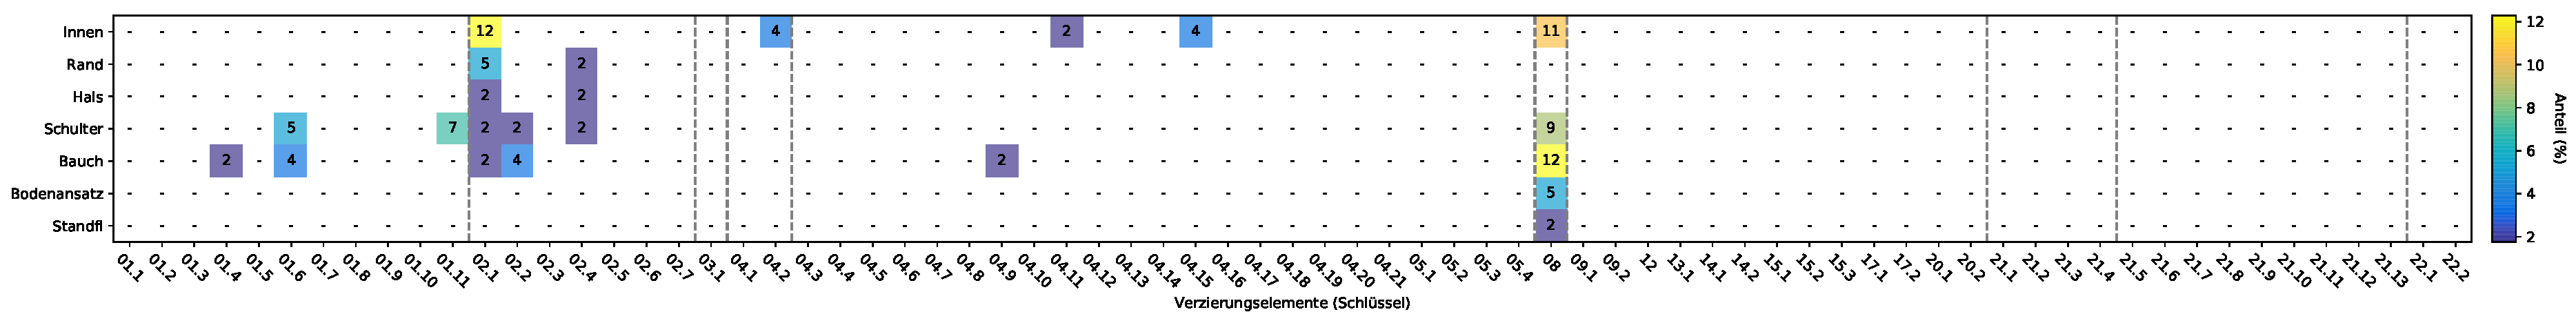
\includegraphics[width=\textwidth]{fig/BKW_Verzierungselmente.pdf}
	\caption*{\textbf{6}\hspace{1em}Bokwango-Gruppe. \vspace{\baselineskip}}
	\label{fig:BKW_Verz}
\end{subfigure}
%\caption{Verzierungselemente: Häufigkeiten.}
\end{sidewaysfigure*}

\addtocounter{figure}{-1}
\begin{sidewaysfigure*}[p]

\centering
\begin{subfigure}{\textwidth}
	\setcounter{subfigure}{6}
	\centering
	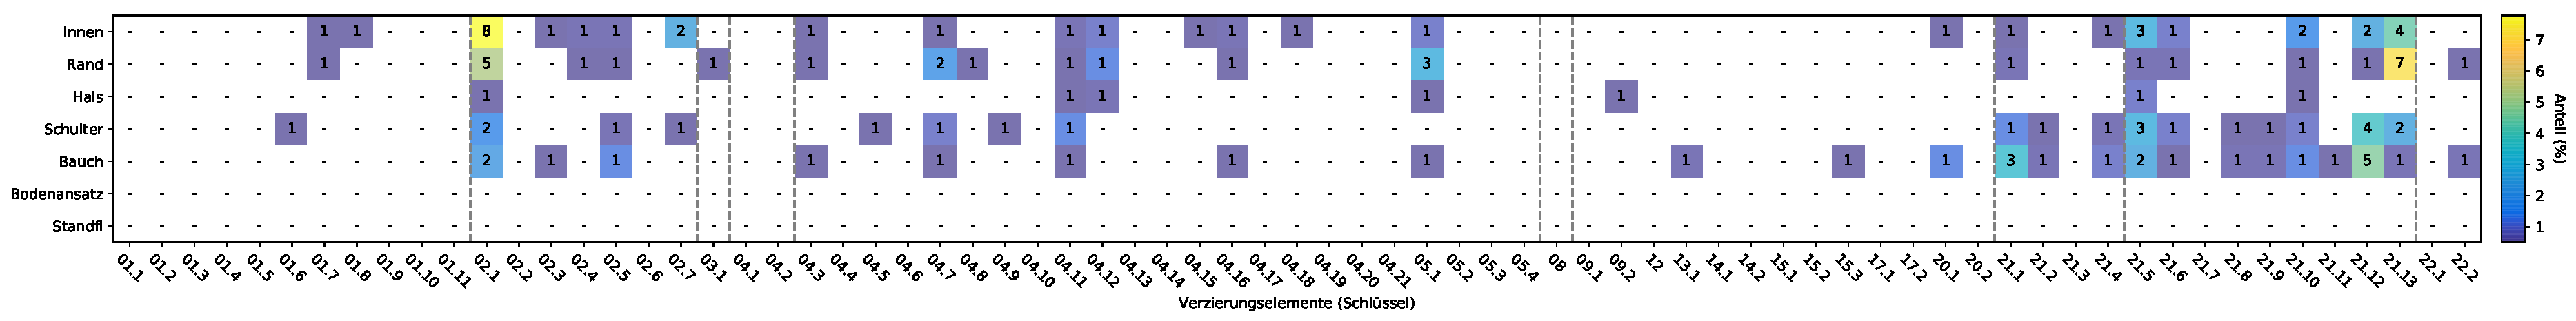
\includegraphics[width=\textwidth]{fig/MTB_Verzierungselmente.pdf}
	\caption*{\textbf{7}\hspace{1em}Motenge-Boma-Gruppe: Verzierungselemente. \vspace{\baselineskip}}
	\label{fig:MTB_Verz}
\end{subfigure}

\begin{subfigure}{\textwidth}
	\centering
	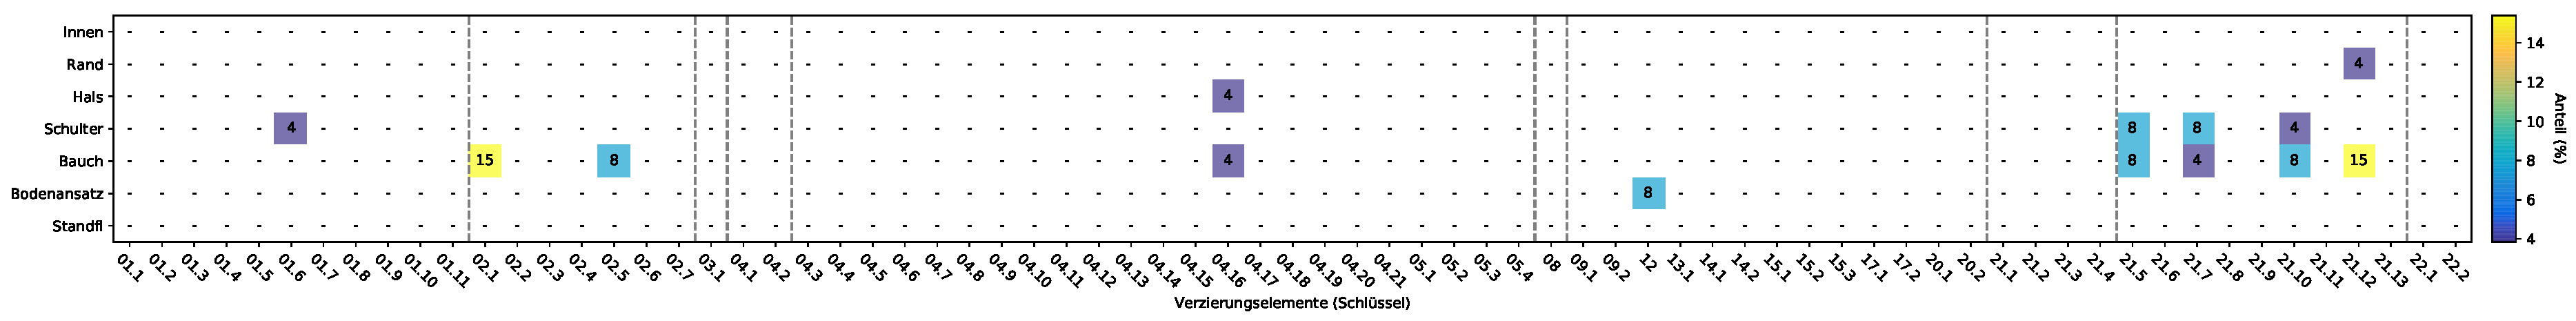
\includegraphics[width=\textwidth]{fig/KPT_Verzierungselmente.pdf}
	\caption*{\textbf{8}\hspace{1em}Kpetene-Gruppe: Verzierungselemente. \vspace{\baselineskip}}
	\label{fig:KPT_Verz}
\end{subfigure}

\begin{subfigure}{\textwidth}
	\centering
	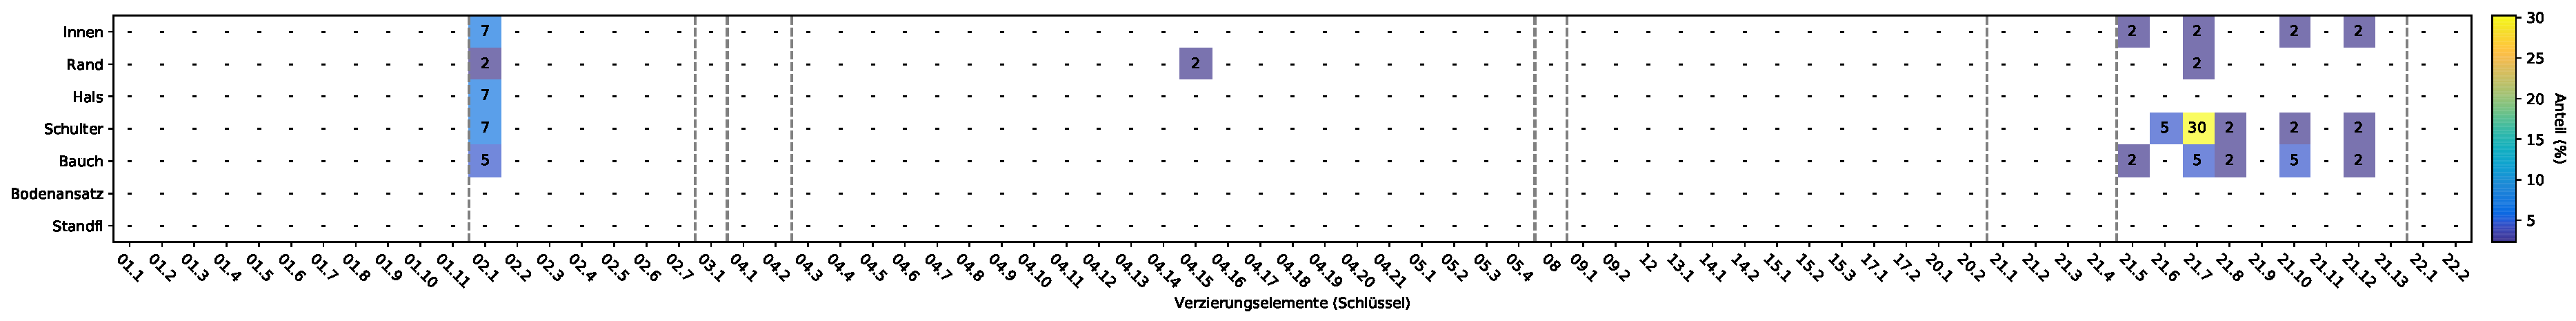
\includegraphics[width=\textwidth]{fig/DAM_Verzierungselmente.pdf}
	\caption*{\textbf{9}\hspace{1em}Dama-Gruppe: Verzierungselemente. \vspace{\baselineskip}}
	\label{fig:DAM_Verz}
\end{subfigure}
%\caption{Verzierungselemente: Häufigkeiten.}
\end{sidewaysfigure*}

\addtocounter{figure}{-1}
\begin{sidewaysfigure*}[p]

\centering
\begin{subfigure}{\textwidth}
	\setcounter{subfigure}{9}
	\centering
	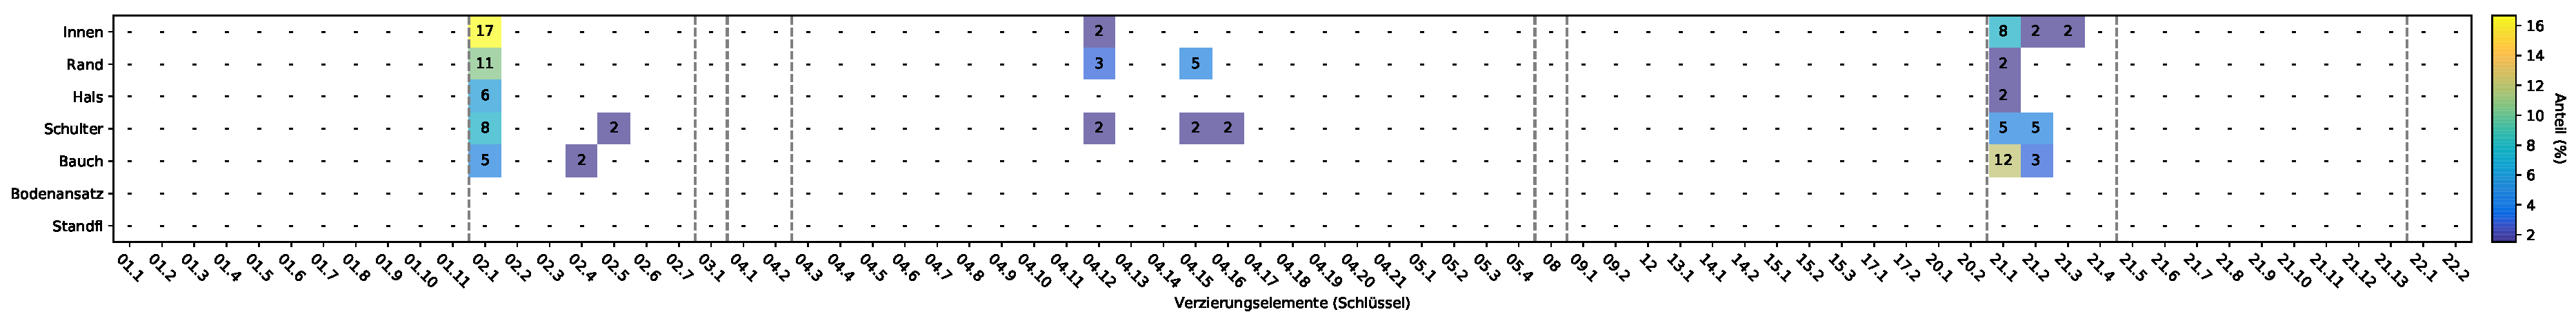
\includegraphics[width=\textwidth]{fig/MBN_Verzierungselmente.pdf}
	\caption*{\textbf{10}\hspace{1em}Mbati-Ngombe-Gruppe: Verzierungselemente. \vspace{\baselineskip}}
	\label{fig:MBN_Verz}
\end{subfigure}

\begin{subfigure}{\textwidth}
	\centering
	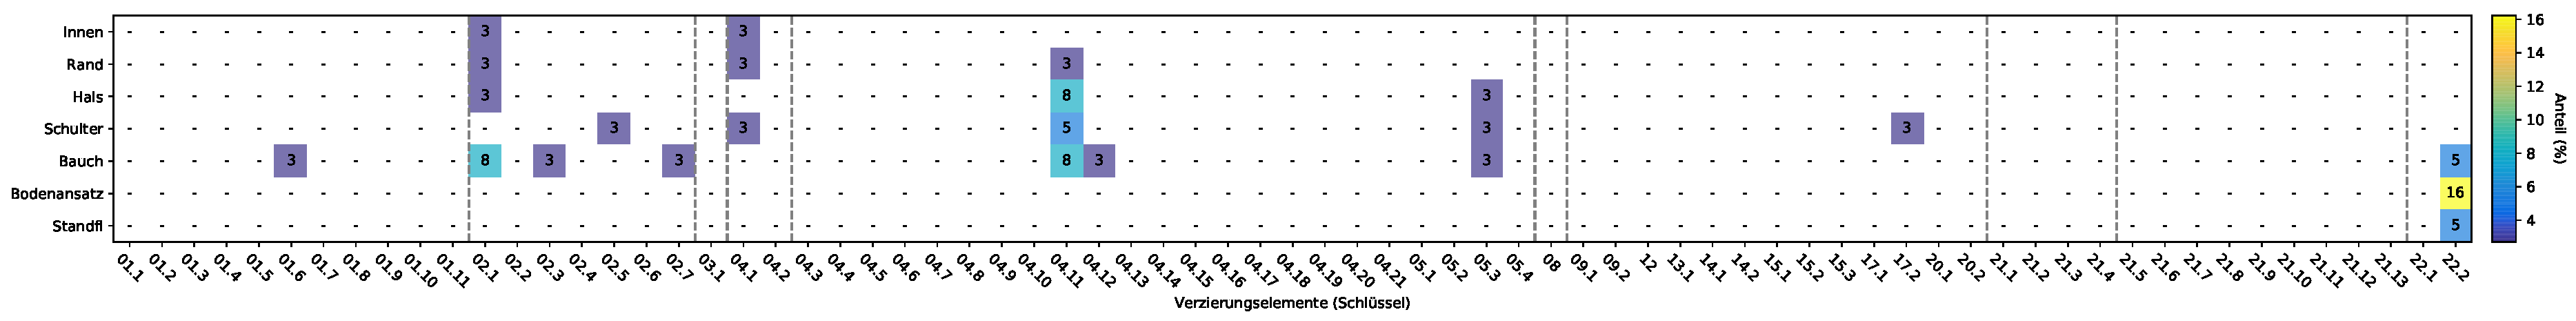
\includegraphics[width=\textwidth]{fig/BAN_Verzierungselmente.pdf}
	\caption*{\textbf{11}\hspace{1em}Bangui-Gruppe: Verzierungselemente. \vspace{\baselineskip}}
	\label{fig:BAN_Verz}
\end{subfigure}

\begin{subfigure}{\textwidth}
	\centering
	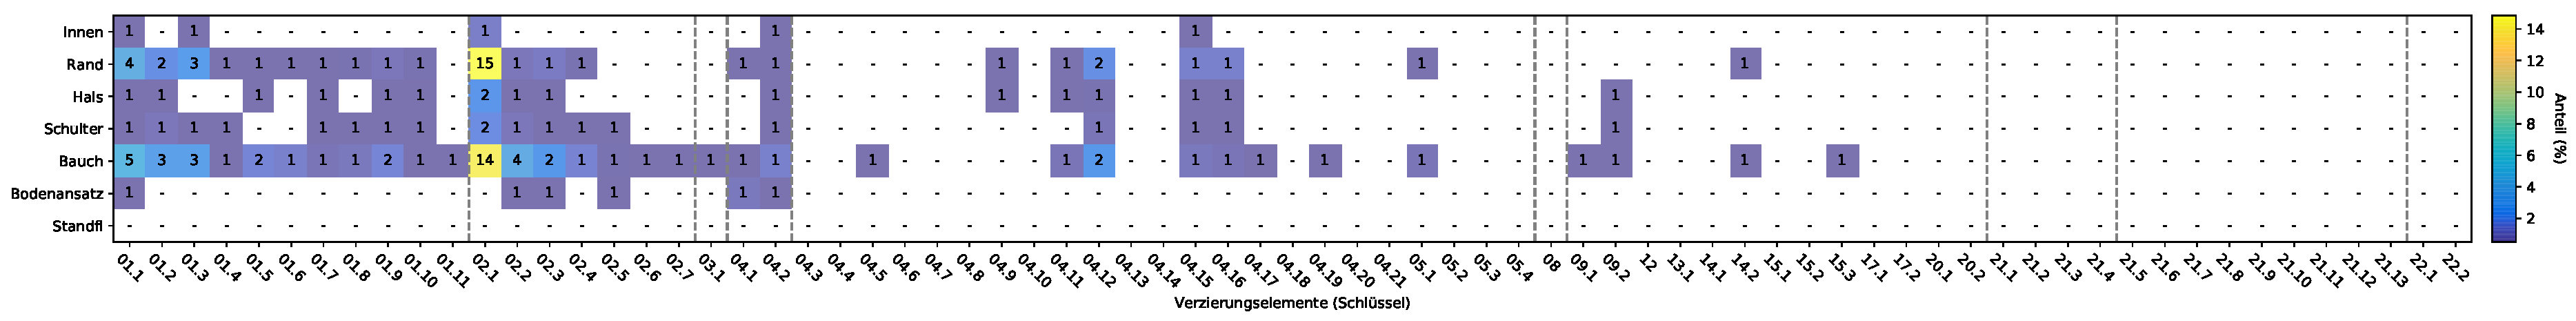
\includegraphics[width=\textwidth]{fig/PKM_Verzierungselmente.pdf}
	\caption*{\textbf{12}\hspace{1em}Pikunda-Munda-Gruppe: Verzierungselemente. \vspace{\baselineskip}}
	\label{fig:PIKMUN_Verz}
\end{subfigure}
%\caption{Verzierungselemente: Häufigkeiten.}
\end{sidewaysfigure*}

\addtocounter{figure}{-1}
\begin{sidewaysfigure*}[p]

\begin{subfigure}{\textwidth}
	\setcounter{subfigure}{12}
	\centering
	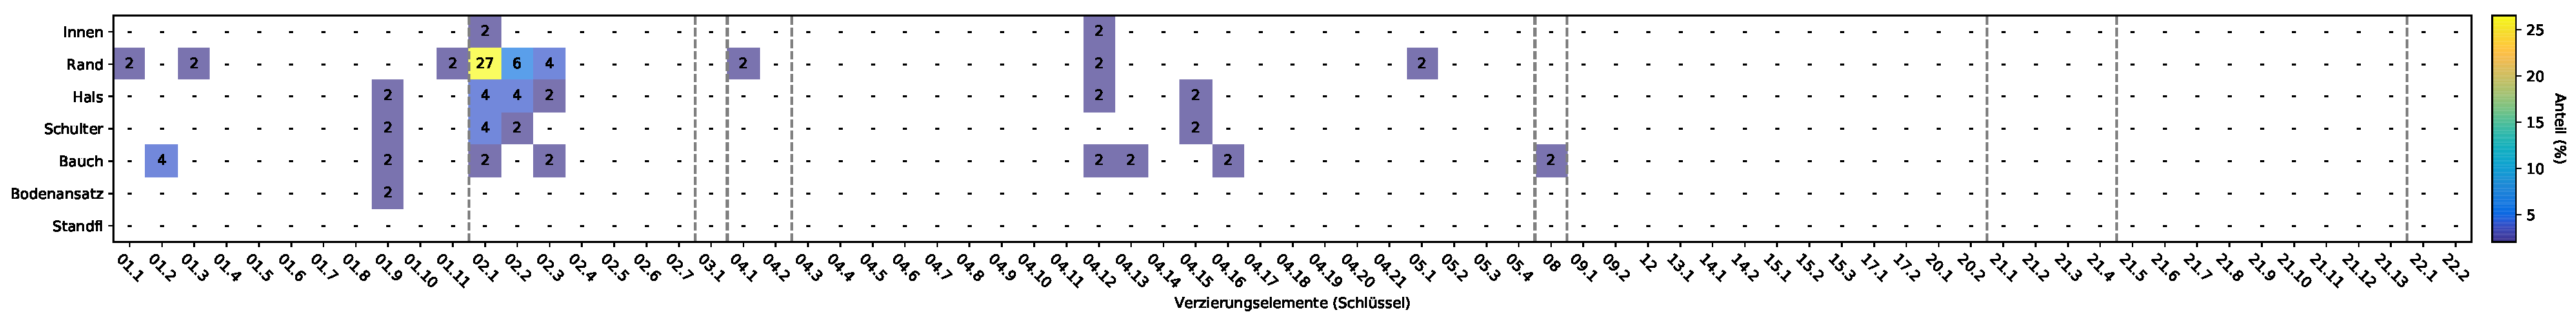
\includegraphics[width=\textwidth]{fig/BOG_Verzierungselmente.pdf}
	\caption*{\textbf{13}\hspace{1em}Bokonongo-Gruppe: Verzierungselemente. \vspace{\baselineskip}}
	\label{fig:BOG_Verz}
\end{subfigure}

\begin{subfigure}{\textwidth}
	\centering
	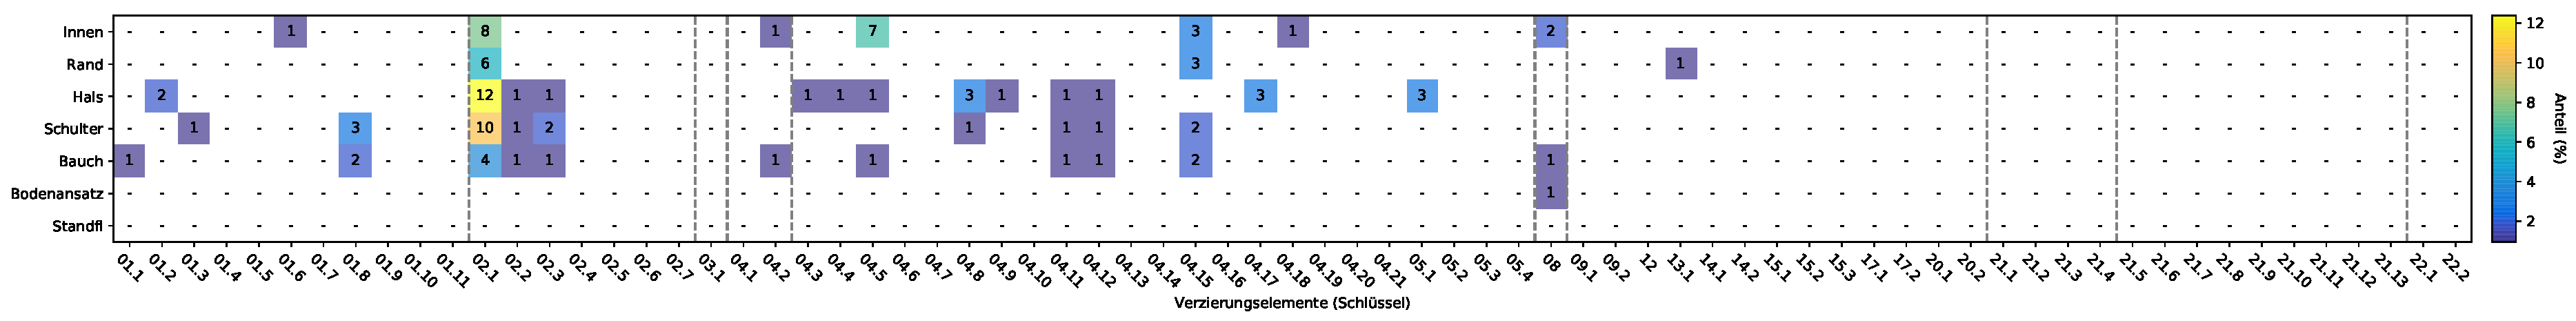
\includegraphics[width=\textwidth]{fig/NGO_Verzierungselmente.pdf}
	\caption*{\textbf{14}\hspace{1em}Ngombe-Gruppe: Verzierungselemente. \vspace{\baselineskip}}
	\label{fig:NGO_Verz}
\end{subfigure}

\begin{subfigure}{\textwidth}
	\centering
	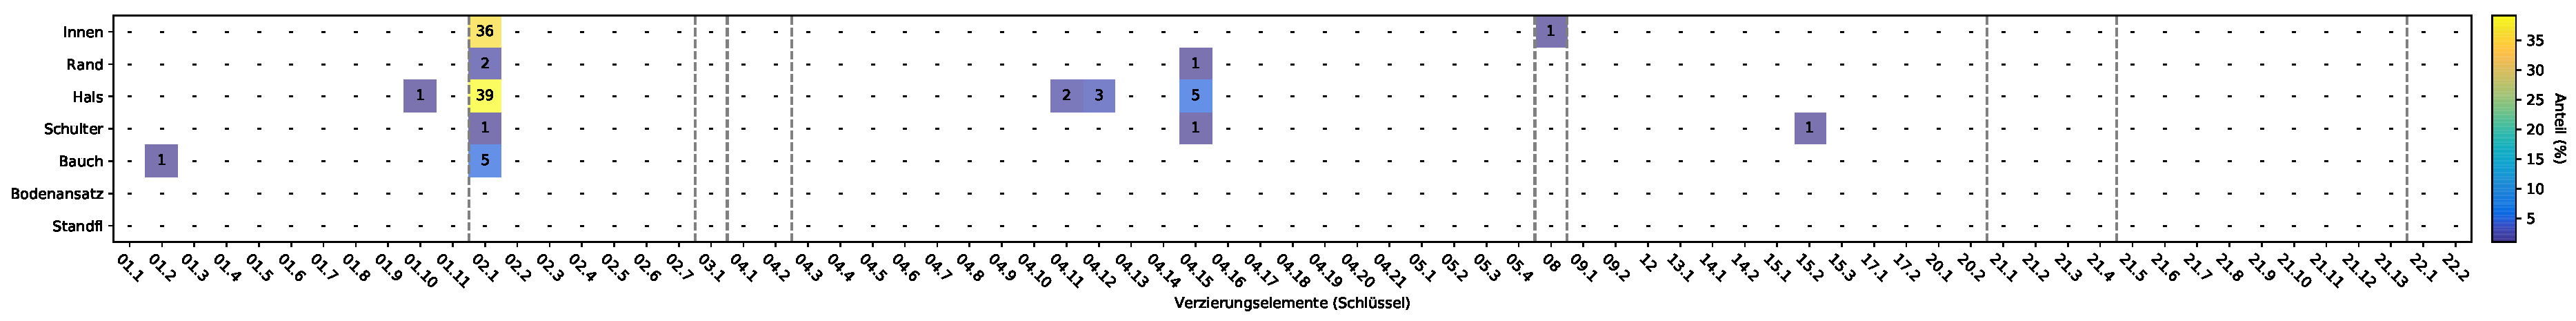
\includegraphics[width=\textwidth]{fig/MAT_Verzierungselmente.pdf}
	\caption*{\textbf{15}\hspace{1em}Matoto-Gruppe: Verzierungselemente. \vspace{\baselineskip}}
	\label{fig:MAT_Verz}
\end{subfigure}
%\caption{Verzierungselemente: Häufigkeiten.}
\end{sidewaysfigure*}

\addtocounter{figure}{-1}
\begin{sidewaysfigure*}[p]

\begin{subfigure}{\textwidth}
	\setcounter{subfigure}{15}
	\centering
	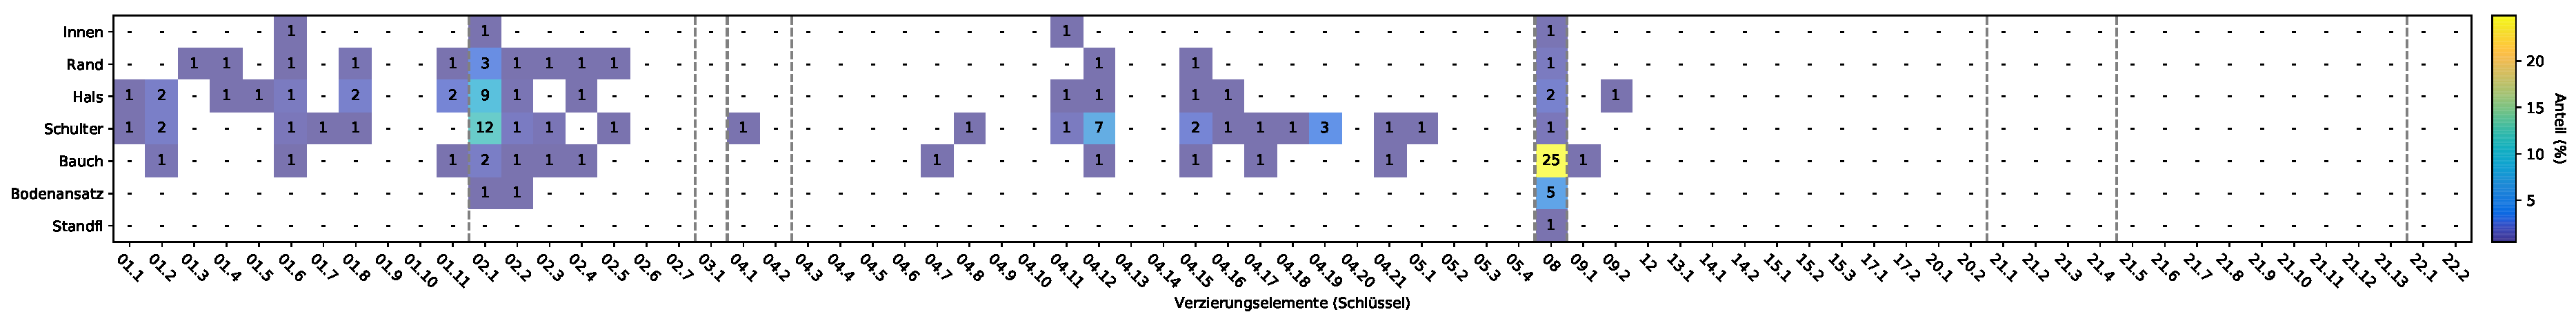
\includegraphics[width=\textwidth]{fig/EBA_Verzierungselmente.pdf}
	\caption*{\textbf{16}\hspace{1em}Ebambe-Gruppe: Verzierungselemente. \vspace{\baselineskip}}
	\label{fig:EBA_Verz}
\end{subfigure}

\begin{subfigure}{\textwidth}
	\centering
	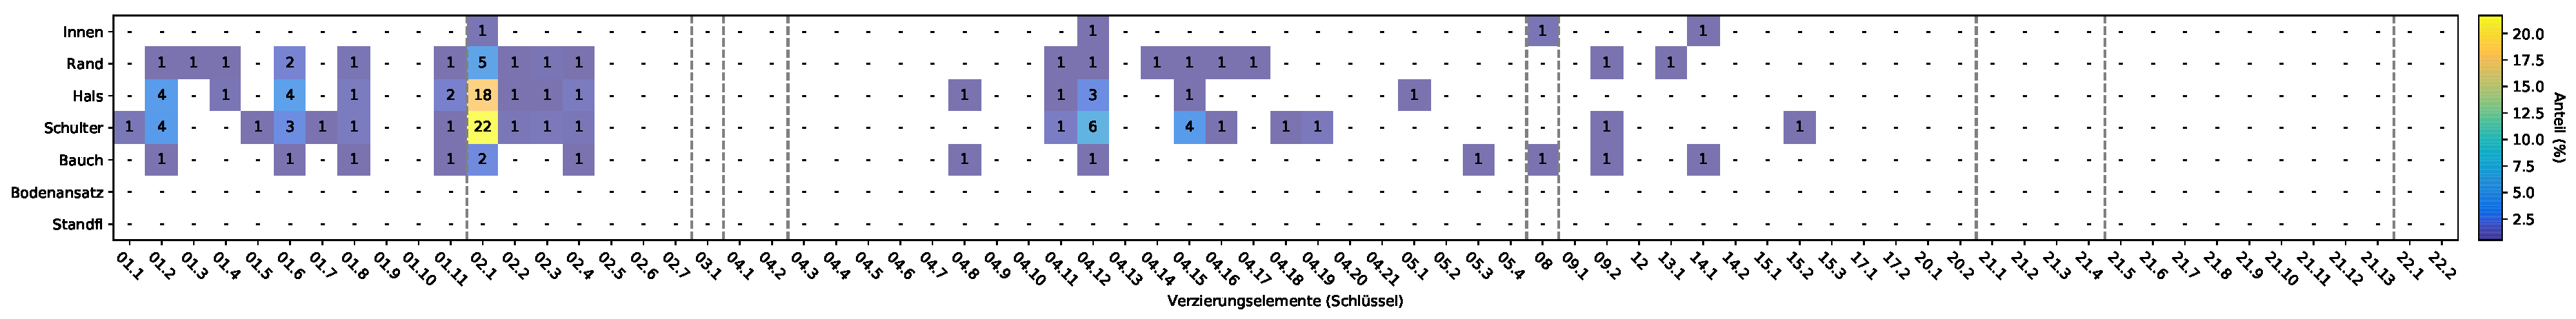
\includegraphics[width=\textwidth]{fig/EPE_Verzierungselmente.pdf}
	\caption*{\textbf{17}\hspace{1em}Epena-Gruppe: Verzierungselemente. \vspace{\baselineskip}}
	\label{fig:EPE_Verz}
\end{subfigure}

\begin{subfigure}{\textwidth}
	\centering
	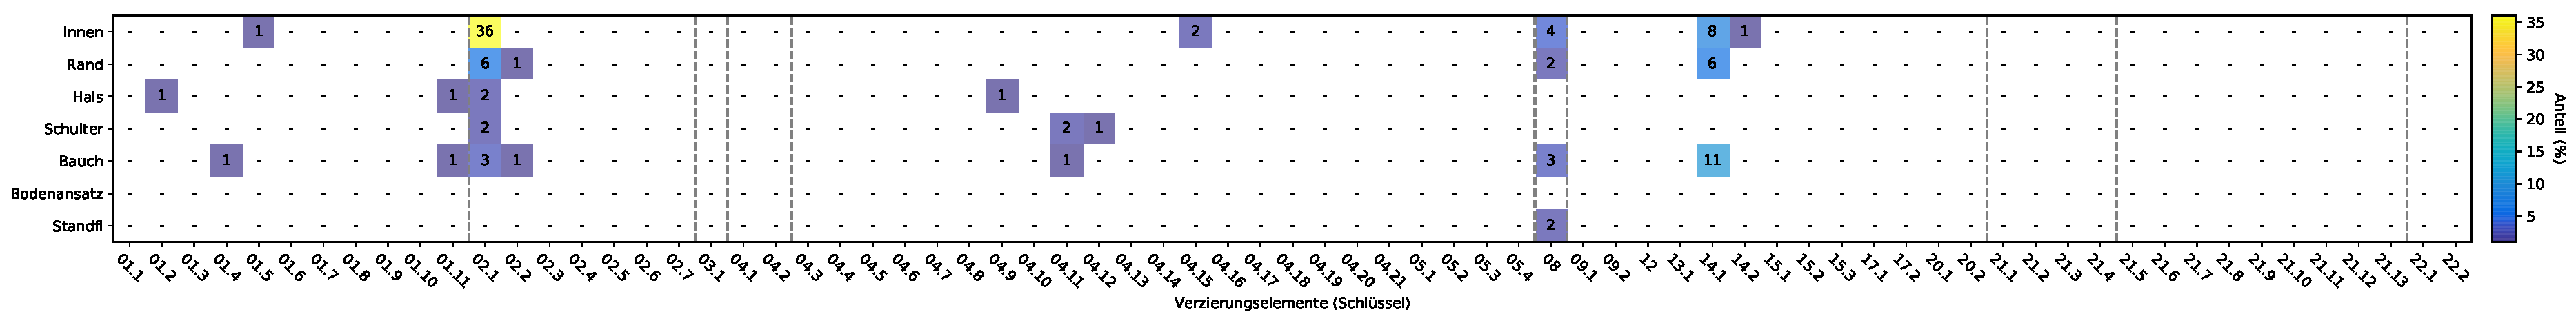
\includegraphics[width=\textwidth]{fig/MKA_Verzierungselmente.pdf}
	\caption*{\textbf{18}\hspace{1em}Mobaka-Gruppe: Verzierungselemente. \vspace{\baselineskip}}
	\label{fig:MKA_Verz}
\end{subfigure}
%\caption{Verzierungselemente: Häufigkeiten.}
\end{sidewaysfigure*}

\addtocounter{figure}{-1}
\begin{sidewaysfigure*}[p]

\begin{subfigure}{\textwidth}
	\setcounter{subfigure}{18}
	\centering
	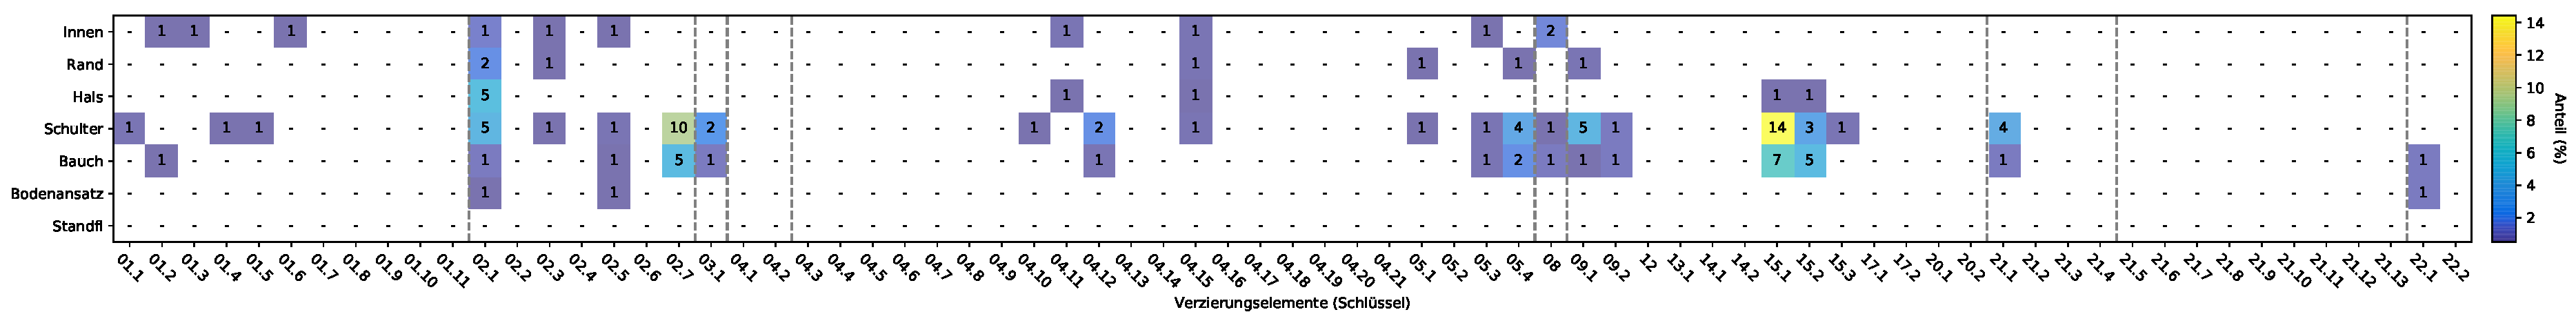
\includegraphics[width=\textwidth]{fig/MDB_Verzierungselmente.pdf}
	\caption*{\textbf{19}\hspace{1em}Mandombe-Gruppe: Verzierungselemente. \vspace{\baselineskip}}
	\label{fig:MDB_Verz}
\end{subfigure}

\begin{subfigure}{\textwidth}
	\centering
	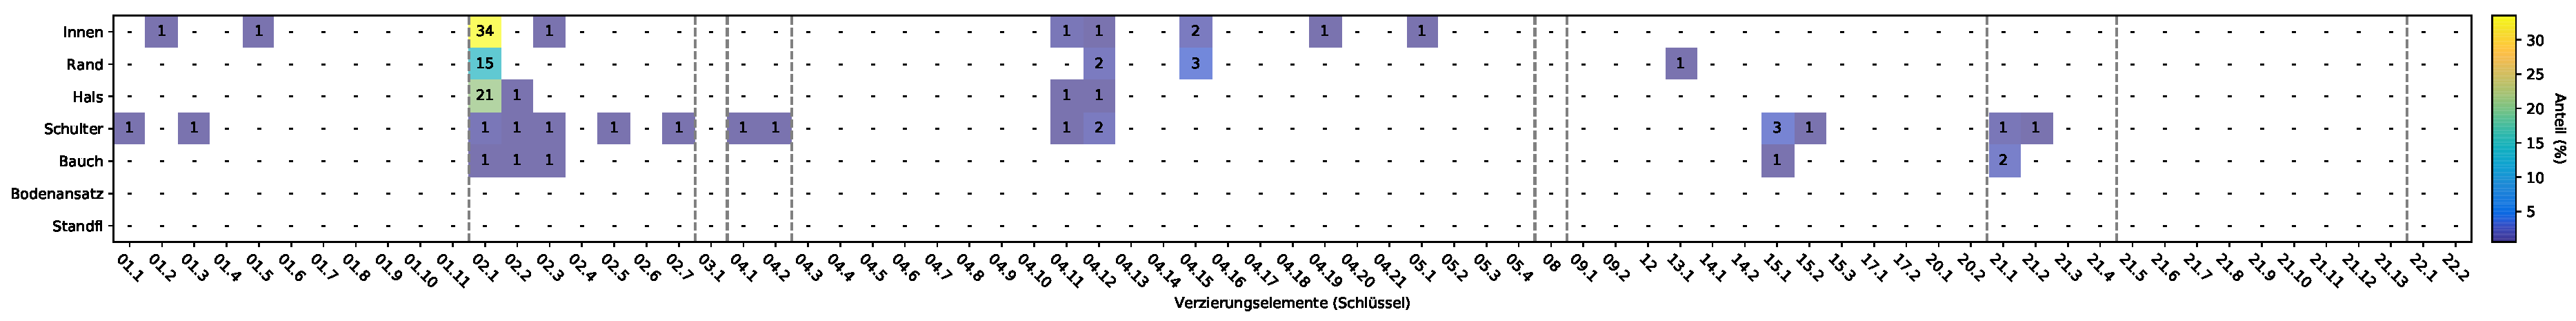
\includegraphics[width=\textwidth]{fig/KON_Verzierungselmente.pdf}
	\caption*{\textbf{20}\hspace{1em}Konda-Gruppe: Verzierungselemente. \vspace{\baselineskip}}
	\label{fig:KON_Verz}
\end{subfigure}

\begin{subfigure}{\textwidth}
	\centering
	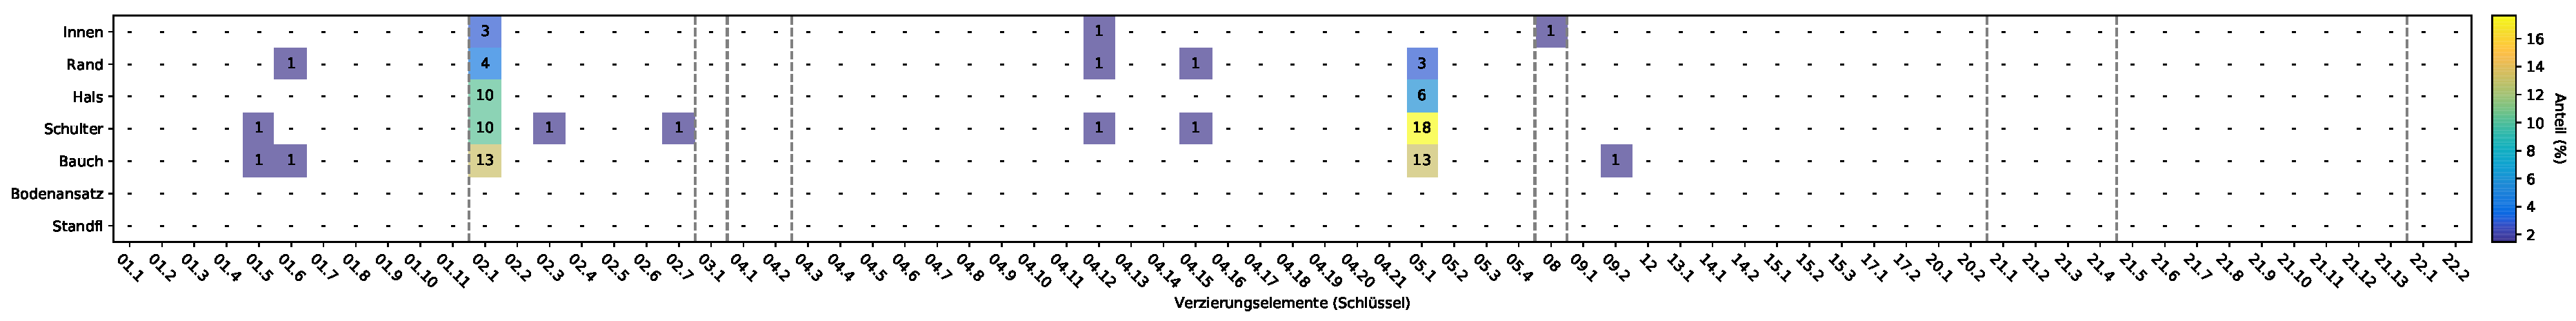
\includegraphics[width=\textwidth]{fig/OUE_Verzierungselmente.pdf}
	\caption*{\textbf{21}\hspace{1em}Ouesso-Gruppe: Verzierungselemente. \vspace{\baselineskip}}
	\label{fig:OUE_Verz}
\end{subfigure}
%\caption{Verzierungselemente: Häufigkeiten.}
\end{sidewaysfigure*}

\addtocounter{figure}{-1}
\begin{sidewaysfigure*}[p]

\begin{subfigure}{\textwidth}
	\setcounter{subfigure}{21}
	\centering
	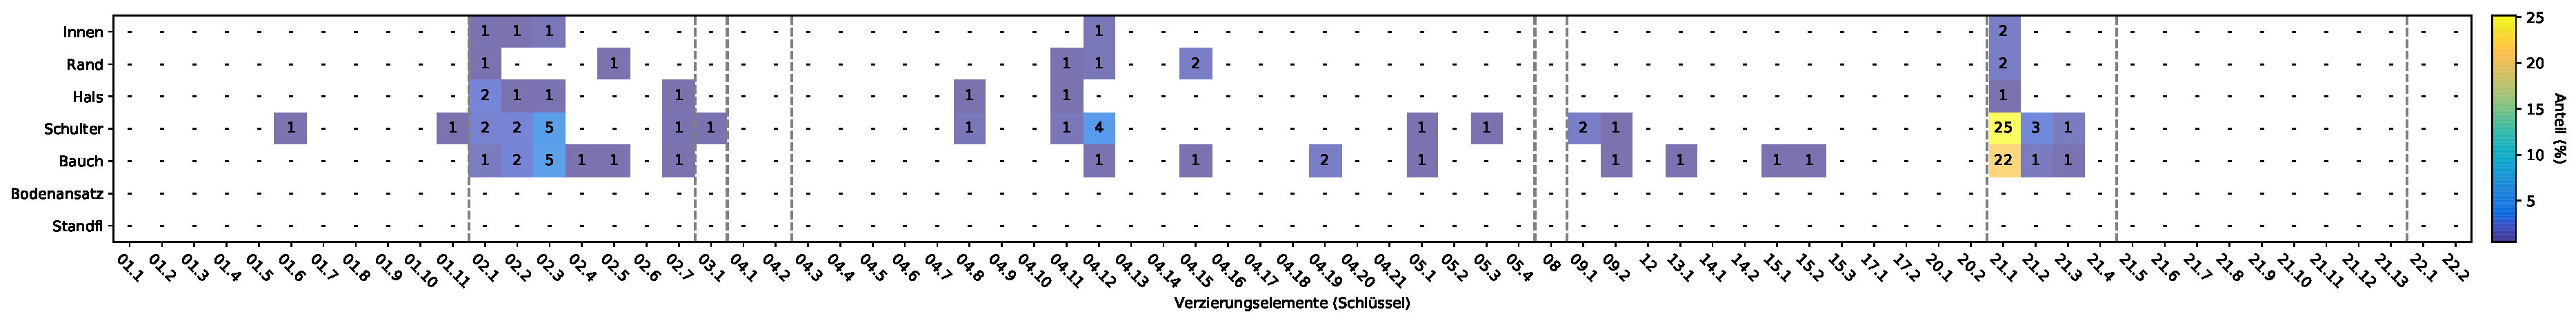
\includegraphics[width=\textwidth]{fig/PDM_Verzierungselmente.pdf}
	\caption*{\textbf{22}\hspace{1em}Pandama-Gruppe: Verzierungselemente. \vspace{\baselineskip}}
	\label{fig:PDM_Verz}
\end{subfigure}

\begin{subfigure}{\textwidth}
	\centering
	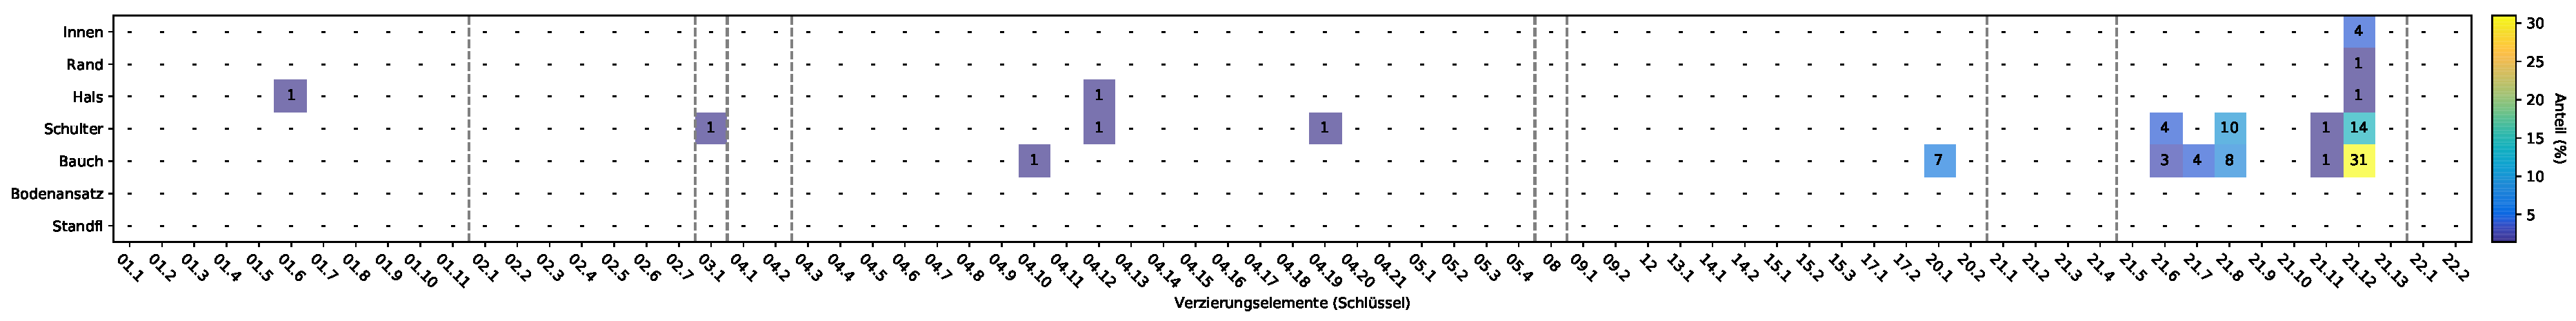
\includegraphics[width=\textwidth]{fig/MBJ_Verzierungselmente.pdf}
	\caption*{\textbf{23}\hspace{1em}Mbenja-Gruppe: Verzierungselemente. \vspace{\baselineskip}}
	\label{fig:MBJ_Verz}
\end{subfigure}

\begin{subfigure}{\textwidth}
	\centering
	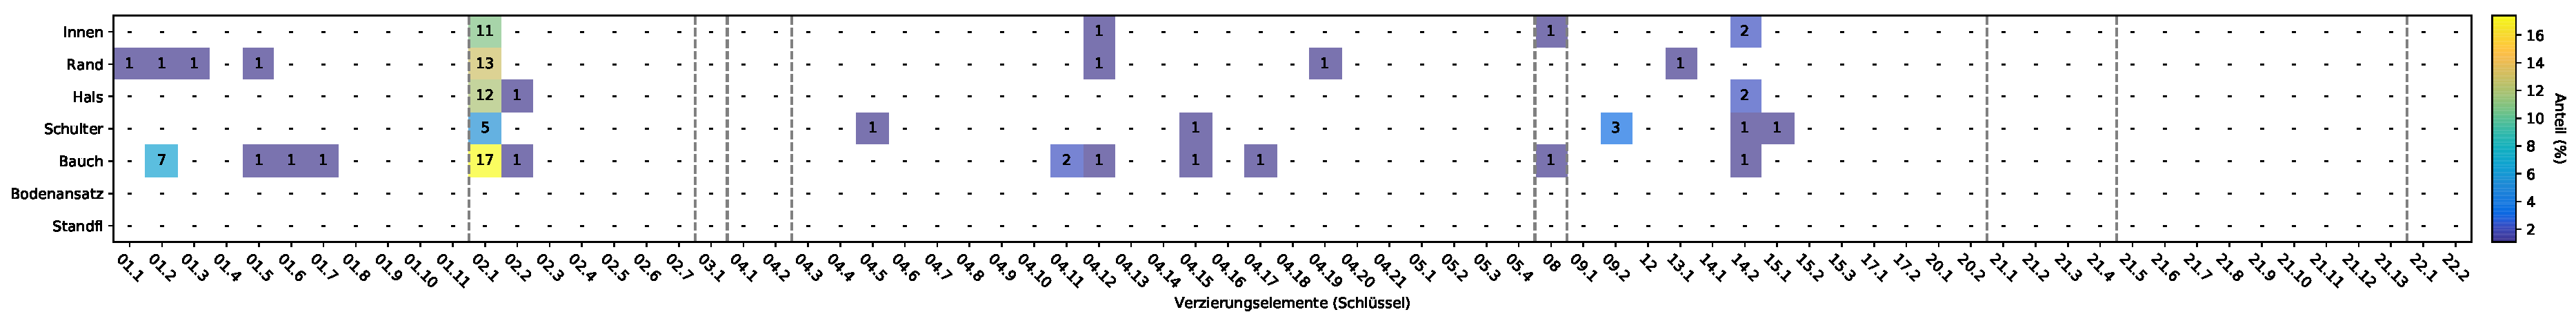
\includegraphics[width=\textwidth]{fig/BBS_Verzierungselmente.pdf}
	\caption*{\textbf{24}\hspace{1em}Bobusa-Gruppe: Verzierungselemente. \vspace{\baselineskip}}
	\label{fig:BBS_Verz}
\end{subfigure}
%\caption{Verzierungselemente: Häufigkeiten.}
\end{sidewaysfigure*}